%************************************************
\chapter[Appendix 2.3: Chapter 2 - Supplementary results]{Appendix 2.3: Chapter 2 - Supplementary results}\label{ch:Appendix2.3}
%************************************************
\renewcommand{\thefigure}{A.2.3.\arabic{figure}}
\setcounter{figure}{0}

\renewcommand{\thetable}{A.2.3.\arabic{table}}
\setcounter{table}{0}

\begin{figure}[ht]
\centering
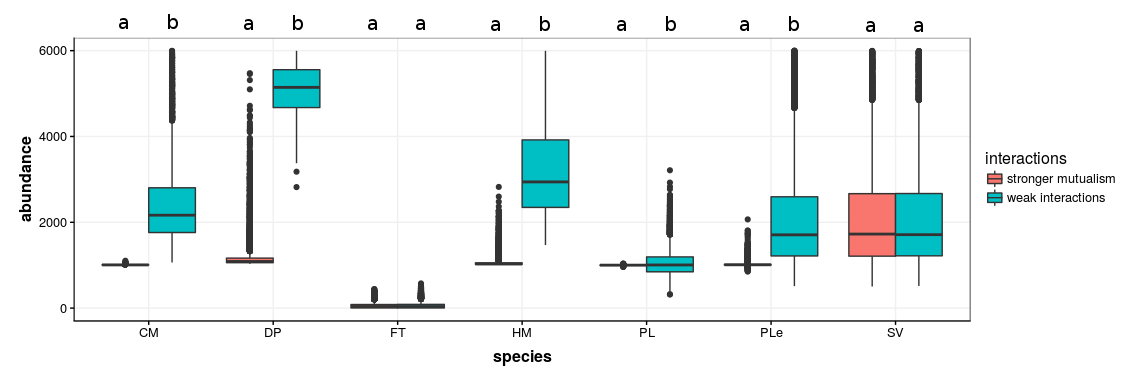
\includegraphics[width=\textwidth]{./Figures/Appendix2_3/Fig_1.png}
\caption[Equal footing equilibrium abundances]{\color{Gray} Equilibrium abundances of the Aire Island community obtained with the equal footing approach (cf. \cref{fig:fig2.2}). Each box represents the distribution of abundances for each species from the 19991 simulations with leading eigenvalue < 0. Simulations with strong antagonistic interactions are not shown since a vast majority of them were unstable. Letters above boxplots indicate significant differences according to Wilcoxon signed-rank tests (CM: W = 19, p < 0.05; DP: W = 12405, p < 0.05; FT: W = 50107000, p = 0.794; HM: W = 58732, p < 0.05; PL: W = 49102000, p < 0.05; PLe: W = 14983000, p < 0.05; SV: W = 49815000, p = 0.649)}
\label{fig:figApp2.3.1}
\end{figure}

\begin{figure}[ht]
\centering
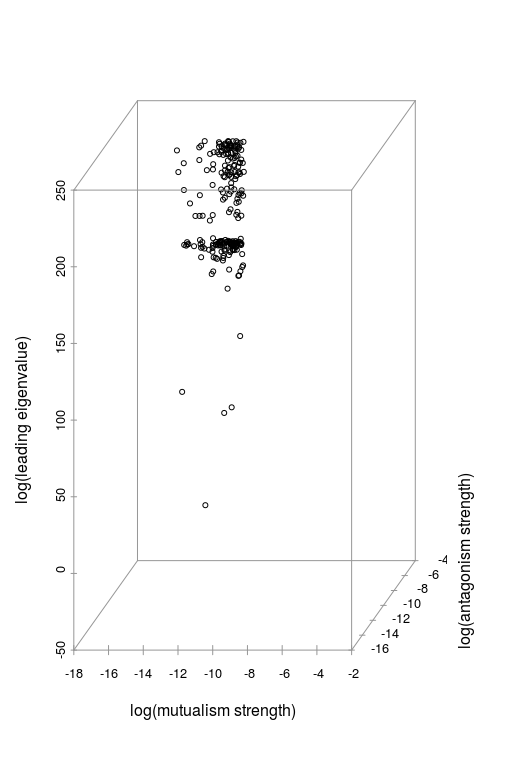
\includegraphics[width=.6\textwidth]{./Figures/Appendix2_3/Fig_2.png}
\caption[Additional equal footing eigenvalues]{\color{Gray} Distribution of the leading eigenvalues of unstable communities modelled with the equal footing approach and not shown in \cref{fig:fig2.3}. In that figure only leading eigenvalues close to 0 where shown for visibility, here, all remaining values have been log-scaled.}
\label{fig:figApp2.3.2}
\end{figure}
